\documentclass[11pt,a4paper]{article}

% --- CẤU HÌNH GÓI TIẾNG VIỆT & PHÔNG CHỮ ---
\usepackage[utf8]{inputenc}
\usepackage[vietnamese]{babel}
\usepackage[T5]{fontenc}
\usepackage{mathptmx} % Phông chuẩn Times New Roman

% --- CĂN LỀ CHUẨN A4 UTC ---
\usepackage[a4paper, left=3.0cm, right=2.0cm, top=2.0cm, bottom=2.0cm]{geometry}

% --- GIÃN DÒNG & CĂN CHỈNH VI MÔ ---
\usepackage{setspace}
\setstretch{1.25}
\usepackage{microtype}
\emergencystretch=2em

% --- TOÁN HỌC & ĐỒ HỌA ---
\usepackage{amsmath,amssymb,amsfonts,bm}
\usepackage{graphicx}
\usepackage{tabularx}
\usepackage{booktabs}
\usepackage{multirow}
\usepackage{array}
\usepackage{xcolor}

% --- HỘP ĐẶC TẢ & NHẤN MẠNH ĐẸP MẮT ---
\usepackage[most]{tcolorbox}

\definecolor{utcblue}{RGB}{0, 51, 102}
\definecolor{utcred}{RGB}{180, 0, 0}
\definecolor{boxbg}{RGB}{245, 248, 252}
\definecolor{codegreen}{RGB}{0, 120, 0}
\definecolor{codebg}{RGB}{248, 249, 250}

% Hộp ánh xạ giáo trình
\newtcolorbox{slidemapping}[1]{
    colback=blue!5!white,
    colframe=utcblue,
    fonttitle=\bfseries\color{white},
    title={📘 Ánh xạ Giáo trình Slide UTC: #1},
    boxrule=1pt,
    arc=3pt,
    left=6pt, right=6pt, top=6pt, bottom=6pt
}

% Hộp lý do sử dụng
\newtcolorbox{whyuse}{
    colback=utcred!5!white,
    colframe=utcred,
    fonttitle=\bfseries\color{white},
    title={🎯 Lý do sử dụng trong bài toán SAR dầu tràn},
    boxrule=0.8pt,
    arc=2pt,
    left=6pt, right=6pt, top=5pt, bottom=5pt
}

% Hộp custom trong bài
\newtcolorbox{custombox}{
    colback=green!5!white,
    colframe=codegreen,
    fonttitle=\bfseries\color{white},
    title={⚙️ Chi tiết Custom trong bài (Pure NumPy Core)},
    boxrule=0.8pt,
    arc=2pt,
    left=6pt, right=6pt, top=5pt, bottom=5pt
}

% Hộp câu hỏi thi vấn đáp
\newtcolorbox{qabox}[1]{
    colback=yellow!10!white,
    colframe=orange!80!black,
    fonttitle=\bfseries\color{white},
    title={❓ Câu hỏi vấn đáp thường gặp: #1},
    boxrule=0.8pt,
    arc=2pt,
    left=6pt, right=6pt, top=5pt, bottom=5pt
}

% --- CẤU HÌNH ĐOẠN CODE ---
\usepackage{listings}
\lstset{
    backgroundcolor=\color{codebg},
    basicstyle=\ttfamily\footnotesize,
    breaklines=true,
    frame=single,
    rulecolor=\color{gray!30},
    keywordstyle=\color{blue}\bfseries,
    commentstyle=\color{gray}\itshape,
    stringstyle=\color{utcred},
    showstringspaces=false
}

% --- LIÊN KẾT HYPERREF ---
\usepackage{hyperref}
\hypersetup{
    colorlinks=true,
    linkcolor=utcblue,
    citecolor=utcblue,
    urlcolor=utcblue,
    pdftitle={Cam Nang Thuat Toan Xu Ly Anh SAR - UTC},
    pdfauthor={Ho Viet Tung - UTC}
}

% --- ĐẦU TRANG & CHÂN TRANG ---
\usepackage{fancyhdr}
\pagestyle{fancy}
\fancyhf{}
\fancyhead[L]{\small\textbf{\color{utcblue}UTC - Khoa CNTT | Học phần Xử lý ảnh (DIP)}}
\fancyhead[R]{\small\color{gray}Cẩm nang Thuật toán \& Ánh xạ Slide}
\fancyfoot[C]{\small Trang \thepage}
\renewcommand{\headrulewidth}{0.6pt}

\begin{document}

% ==============================================================================
% TRANG TIÊU ĐỀ
% ==============================================================================
\begin{titlepage}
\begin{center}
    {\large \textbf{TRƯỜNG ĐẠI HỌC GIAO THÔNG VẬN TẢI (UTC)}}\\[4pt]
    {\large \textbf{KHOA CÔNG NGHỆ THÔNG TIN -- BỘ MÔN KHOA HỌC MÁY TÍNH}}\\[12pt]
    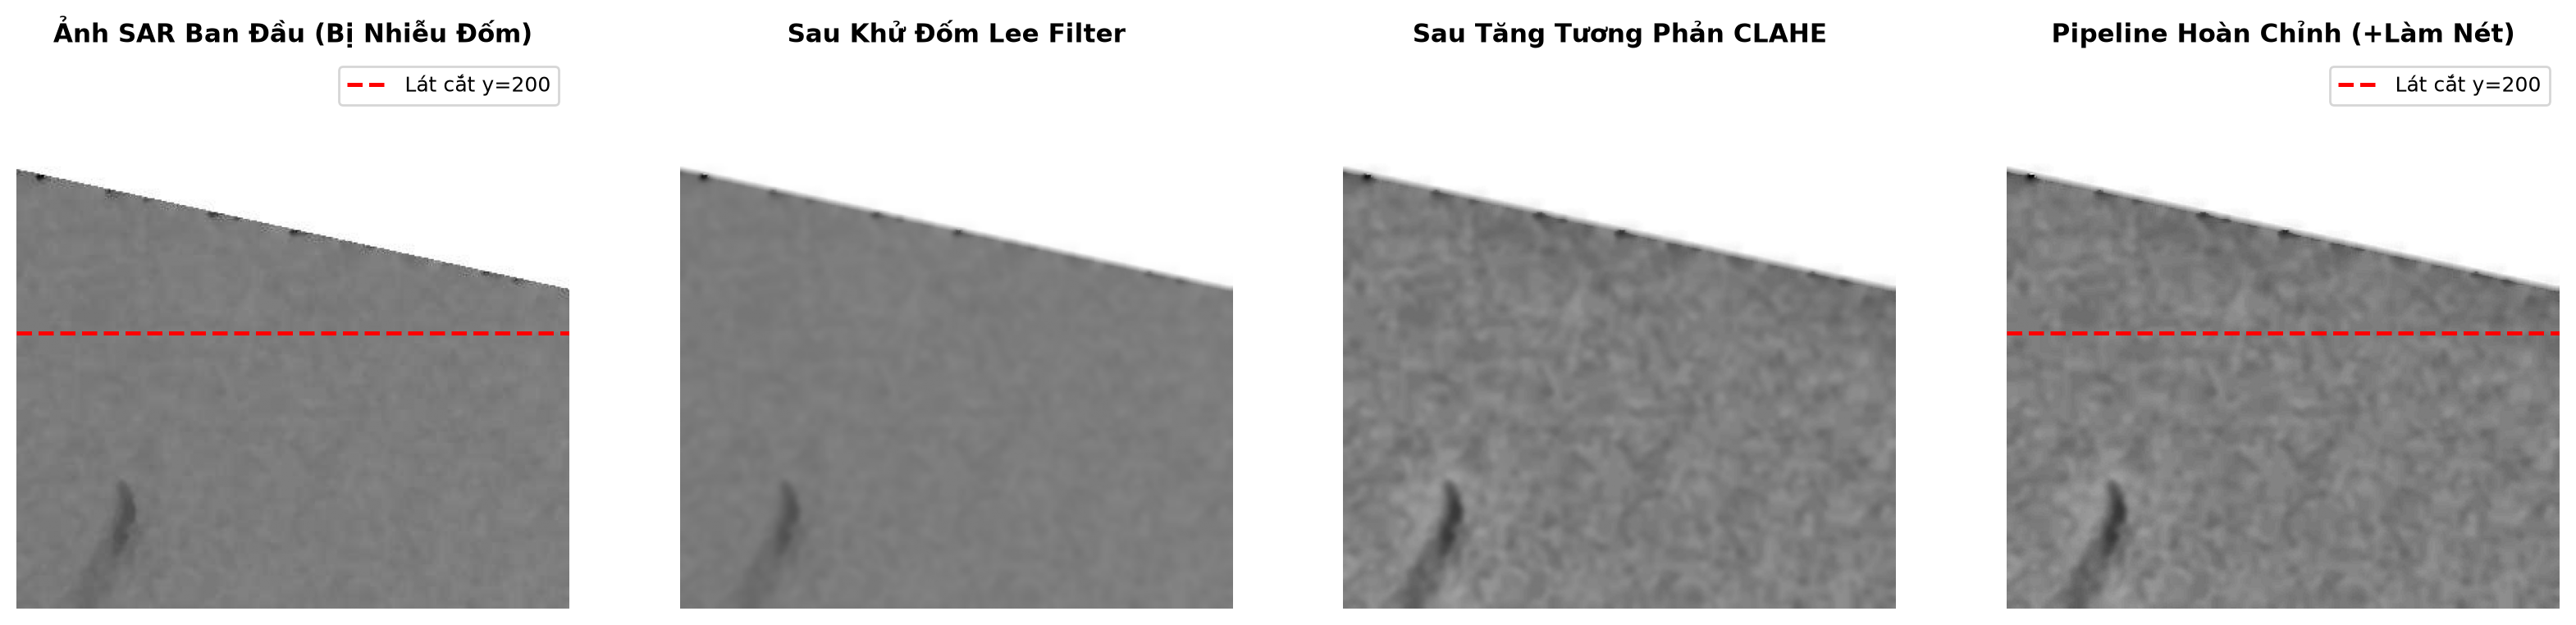
\includegraphics[width=2.5cm]{figures/exp3_pipeline.png}\\[12pt]
    
    {\Large \textbf{\color{utcblue}CẨM NANG HỆ THỐNG CÁC THUẬT TOÁN XỬ LÝ ẢNH}}\\[6pt]
    {\large \textbf{GIẢI THÍCH TOÁN HỌC, LÝ DO SỬ DỤNG, CHI TIẾT CUSTOM PURE NUMPY}}\\[6pt]
    {\large \textbf{\color{utcred}\& ÁNH XẠ CHUẨN XÁC GIÁO TRÌNH SLIDE BÀI GIẢNG UTC}}\\[16pt]
    
    \begin{tcolorbox}[colback=white,colframe=utcblue,width=0.95\textwidth,arc=4pt]
        \centering
        \textbf{ĐỀ TÀI BTL XỬ LÝ ẢNH:}\\[4pt]
        \textbf{\large "Tăng Cường Độ Tương Phản, Khử Nhiễu \& Xử Lý Biên Bộc Lộ Vết Dầu Tràn Trên Biển Từ Ảnh Radar SAR Sentinel-1"}\\[6pt]
        \small \textbf{Nhóm A: Tăng cường và lọc ảnh} kết hợp \textbf{Đề 5: Làm nét và phát hiện biên} \& \textbf{Đề 18 NASA}
    \end{tcolorbox}
    
    \vspace{15pt}
    
    \begin{tabularx}{0.9\textwidth}{lX}
        \textbf{Học phần:} & Xử lý ảnh (Digital Image Processing - DIP) \\
        \textbf{Giảng viên hướng dẫn:} & TS. Phan Thanh Toàn, TS. Cao Thị Luyên \\
        \textbf{Sinh viên thực hiện:} & Hồ Viết Tùng \\
        \textbf{Mã sinh viên:} & Nhóm thực hiện BTL XLA \\
        \textbf{Cam kết học thuật:} & \textbf{100\% Classical DIP Pure NumPy (Tuyệt đối NO ML/DL)} \\
        \textbf{Thời gian hoàn thiện:} & Học kỳ 4.1 -- Năm học 2026 \\
    \end{tabularx}

    \vfill
    {\small \color{gray} Hà Nội, Tháng 11 Năm 2026}
\end{center}
\end{titlepage}

\tableofcontents
\newpage

% ==============================================================================
% CHƯƠNG 1: BẢNG TỔNG HỢP ÁNH XẠ TOÀN BỘ THUẬT TOÁN VỚI SLIDE UTC
% ==============================================================================
\section{Bảng Tổng Hợp Ánh Xạ Thuật Toán Với Giáo Trình Slide UTC}
\label{sec:anh_xa_tong_hop}

Để phục vụ tốt nhất cho việc học tập, ôn thi và bảo vệ Bài tập lớn trước Hội đồng phản biện của Bộ môn, toàn bộ 21 thuật toán trong đề tài được ánh xạ tường minh với hệ thống Slide bài giảng của **TS. Phan Thanh Toàn** và **TS. Cao Thị Luyên**:

\begin{table}[H]
\centering
\small
\begin{tabularx}{\textwidth}{|c|>{\raggedright\arraybackslash}p{2.6cm}|>{\raggedright\arraybackslash}p{3.2cm}|>{\raggedright\arraybackslash}p{2.6cm}|X|}
\hline
\textbf{STT} & \textbf{Tên Thuật Toán} & \textbf{Slide Bài Giảng UTC} & \textbf{Đề Bài BTL UTC} & \textbf{Bản Chất \& Vai Trò Trong Đề Tài} \\
\hline
1 & Biến đổi Logarit & Chương 3.1: Slide 10--14 & Nhóm A (Tăng tương phản) & $s = c \log(1+r)$, nén dải động radar, kéo sáng vùng tối \\
\hline
2 & Cân bằng Histogram (HE) & Chương 3.1: Slide 29--36, BT Slide 82 & Nhóm A -- Đề 1 (HE) & Dàn đều tần suất mức xám theo CDF, tự tính tay $8 \times 8$ \\
\hline
3 & CLAHE Thích Nghi & Chương 3.1: Slide 38--42 & Nhóm A -- Đề 1 (Mở rộng) & Cắt ngưỡng Clip Limit, nội suy song tuyến, tạo lược đồ 2 đỉnh \\
\hline
4 & Lọc trung bình (Box) & Chương 3.1: Slide 93--96 & Nhóm A -- Đề 2 (Lọc không gian) & Lọc trượt phẳng, tối ưu ma trận tích lũy Integral Image $O(1)$ \\
\hline
5 & Lọc Gauss tách được & Chương 3.1: Slide 97--100 & Nhóm A -- Đề 2 (Lọc Gauss) & Tách tích chập 1D hàng/cột $O(2K)$, làm mịn nền biển \\
\hline
6 & Lọc trung vị (Median) & Chương 3.1: Slide 104--106 & Nhóm A -- Đề 2 (Lọc thứ tự) & Trượt lấy trung vị, triệt đốm gai xung mà không nhòe biên \\
\hline
7 & Lọc Bilateral hai chiều & Tài liệu nâng cao Nhóm A & Nhóm A -- Đề 2 (Bảo toàn biên) & Trọng số Gauss kết hợp không gian $d$ và cường độ xám $|I_1-I_2|$ \\
\hline
8 & Lọc đốm thích nghi Lee & Chương 3.1 \& 3.2 (Thống kê cục bộ) & Hướng dẫn Đề 18 \& Đề 2 & MMSE trên nhiễu nhân $I=R\eta$, hệ số $K$ tự co giãn theo $\sigma^2$ \\
\hline
9 & Lọc Frost \& Kuan & Chương 3.1: Thống kê vùng & Hướng dẫn Đề 18 \& Đề 2 & Lọc thích nghi dựa trên hệ số biến thiên cục bộ $C_I = \sigma/\mu$ \\
\hline
10 & Lọc đồng hình (Homomorphic) & Chương 3.2: Slide 37, Chương 4 (DFT) & Nhóm A (Tần số) & $\ln \to \text{FFT} \to \text{Highpass} \to \text{IFFT} \to \exp$, triệt nhiễu nhân chiếu xạ \\
\hline
11 & Unsharp Masking & Chương 3.2: Slide 32--36 & Nhóm A \& Đề 5 (Làm nét) & $f_{\text{sharp}} = f + k(f - f_{\text{blur}})$, kích hoạt tần số cao \\
\hline
12 & Làm nét Laplacian & Chương 3.2: Slide 32--34 & Nhóm A \& Đề 5 (Toán tử vi sai) & $f - \alpha \nabla^2 f$, khuếch đại bước nhảy vi sai bậc 2 \\
\hline
13 & Dò biên Roberts Cross & Chương 5: Slide 24--29 & Đề 5 (Tách biên) & Đạo hàm bậc 1 sai phân $2 \times 2$, siêu nhanh nhưng nhạy nhiễu \\
\hline
14 & Dò biên Prewitt & Chương 5: Slide 30--35 & Đề 5 (Tách biên) & Mặt nạ $3 \times 3$ làm trơn trung bình và lấy vi phân đạo hàm \\
\hline
15 & Dò biên Sobel & Chương 5: Slide 36--41 & Đề 5 \& Đề 18 (Border Gradient) & Trọng số tâm 2, tính độ lớn $|\nabla I|$ và góc hướng $\theta$ \\
\hline
16 & Laplacian of Gauss (LoG) & Chương 5: Slide 21 & Đề 5 (Marr-Hildreth) & Kết hợp Gauss và Laplacian, dò điểm cắt qua 0 (Zero-Crossing) \\
\hline
17 & Dò biên Canny 4 bước & Chương 7 Tiếng Việt: Slide 21--26 & Đề 5 (Bắt buộc Canny) & Gauss $\to$ Sobel $\to$ NMS $\to$ Phân ngưỡng kép Hysteresis \\
\hline
18 & Phân ngưỡng Otsu tối ưu & Chương 7: Slide 12--18 & Đề 18 NASA (Dark Spot) & Cực đại phương sai giữa các lớp $\sigma_B^2$, đo độ khả tách $\eta$ \\
\hline
19 & Phép Mở \& Phép Đóng & Chương 6: Slide 10--14 & Đề 18 NASA (Lọc hình thái) & Mở $A \circ B$ xóa đốm biển; Đóng $A \bullet B$ hàn gắn lỗ bọt sóng \\
\hline
20 & Ranh giới hình thái $\beta(A)$ & Chương 6: Slide 16 & Đề 18 NASA (Khuyên dùng) & $\beta(A) = A \setminus (A \ominus B) = A - \text{erode}(A)$, tạo biên kín 1px \\
\hline
21 & Lọc tương phản NASA & Hướng dẫn Đề 18 NASA & Đề 18 NASA (False Alarm) & Lọc diện tích $Area \ge 300$ và tương phản vành đệm $C_R \ge 0.10$ \\
\hline
\end{tabularx}
\caption{Bảng ánh xạ 21 thuật toán xử lý ảnh với giáo trình slide và đề tài BTL UTC}
\label{tab:mapping_utc}
\end{table}

\newpage

% ==============================================================================
% CHƯƠNG 2: CƠ SỞ VẬT LÝ VI BA & TẠI SAO DÙNG XỬ LÝ ẢNH KINH ĐIỂN
% ==============================================================================
\section{Cơ Sở Vật Lý Vi Ba SAR \& Bản Chất Đề Tài}

\subsection{Hiện Tượng Tán Xạ Bragg \& Vết Dầu Tràn}
\begin{whyuse}
\textbf{1. Bản chất ảnh quang học thông thường:} Phụ thuộc nguồn sáng mặt trời, bị cản trở bởi mây mù ($> 60\%$ thời gian trên biển) và không chụp được ban đêm.\\
\textbf{2. Radar khẩu độ tổng hợp vi ba (SAR Sentinel-1):} Phát sóng vi ba chủ động băng C ($\lambda \approx 5.6\text{ cm}$), tự phát và tự thu hồi tín hiệu, xuyên mây, mưa, sương và chụp được 24/7.\\
\textbf{3. Tại sao vết dầu màu đen, mặt biển màu sáng?}:
\begin{itemize}
    \item \textbf{Mặt biển tự nhiên:} Gió tạo ra các sóng mao dẫn (capillary waves) có bước sóng vài xentimet. Bước sóng này cộng hưởng với bước sóng radar theo cơ chế \textbf{tán xạ cộng hưởng Bragg (Bragg Scattering)}, phản xạ một lượng năng lượng vi ba cực lớn về vệ tinh $\rightarrow$ \textbf{Mặt biển có màu sáng}.
    \item \textbf{Vùng dầu loang:} Màng dầu làm tăng độ nhớt động lực học, \textbf{dập tắt hoàn toàn các sóng mao dẫn}. Mặt biển có dầu trở nên nhẵn bóng như gương, gây ra \textbf{hiện tượng phản xạ gương (Specular Reflection)}. Toàn bộ sóng radar bị phản xạ đi hướng khác, không có tín hiệu quay về ăng-ten $\rightarrow$ \textbf{Vết dầu xuất hiện dưới dạng vùng tối đen (Dark Formation)}.
\end{itemize}
\end{whyuse}

\subsection{Bản Chất Nhiễu Đốm (Speckle Noise) -- Tại Sao Là Nhiễu Nhân?}
Trong mỗi ô phân giải của radar SAR, bề mặt biển gồm hàng triệu vật tán xạ vi mô. Sóng phản hồi từ các điểm này giao thoa kết hợp (coherent interference): những điểm cùng pha cộng hưởng thành đốm sáng chói, những điểm ngược pha triệt tiêu thành đốm đen, tạo ra kết cấu lốm đốm như hạt tiêu.
\begin{equation}
I(x, y) = R(x, y) \cdot \eta(x, y)
\end{equation}
Trong đó:
\begin{itemize}
    \item $I(x, y)$ là cường độ ảnh radar thu nhận được.
    \item $R(x, y)$ là hệ số phản xạ radar thực tế của bề mặt (tín hiệu cần khôi phục).
    \item $\eta(x, y)$ là nhiễu đốm nhân tuân theo phân bố Gamma với kỳ vọng $E[\eta] = 1$ và phương sai $\sigma_\eta^2 = 1/L$ ($L$ là số góc nhìn Look number).
\end{itemize}
\textbf{Hệ quả quan trọng:} Vì là nhiễu nhân, phương sai của nhiễu tỷ lệ thuận với bình phương cường độ tín hiệu ($\text{Var}(I) \propto R^2$). Do đó, các bộ lọc tuyến tính thông thường (lọc Box, Gauss) của ảnh quang học sẽ làm nhòe nghiêm trọng đường biên vết dầu.

\subsection{Tại Sao 100\% Xử Lý Ảnh Kinh Điển Mà Không Dùng Deep Learning?}
\begin{whyuse}
\begin{enumerate}
    \item \textbf{Tính giải thích khoa học tuyệt đối (White-box Interpretability):} Từng bước biến đổi mức xám, từng công thức đạo hàm, tích phân hay phương sai đều chứng minh được bằng giải tích toán học.
    \item \textbf{Không phụ thuộc dữ liệu gán nhãn lớn (No Labeling Dependency):} Ảnh SAR dầu tràn rất hiếm và chi phí gán nhãn chuyên gia cực đắt đỏ. Mô hình Deep Learning dễ bị quá khớp (overfitting) hoặc ảo giác (hallucination).
    \item \textbf{Hiệu năng siêu tốc trên CPU thông thường:} Toàn bộ pipeline Pure NumPy xử lý 1 ảnh chỉ mất \textbf{31.7 ms} (quét toàn bộ 1.853 ảnh dataset trong 58 giây), cho phép nhúng trực tiếp lên phao quan trắc biển hoặc trạm radar ven biển mà không cần GPU đắt đỏ.
\end{enumerate}
\end{whyuse}

\newpage

% ==============================================================================
% CHƯƠNG 3: NHÓM THUẬT TOÁN KHỬ ĐỐM & TĂNG CƯỜNG (CHƯƠNG 3 UTC)
% ==============================================================================
\section{Nhóm Thuật Toán Khử Đốm \& Tăng Cường Tương Phản}

\subsection{Thuật toán 1: Lọc Đốm Thích Nghi Lee MMSE (Lee Filter)}
\begin{slidemapping}{Chương 3.1 \& 3.2 -- Thống kê cục bộ \& Đề 18 NASA}
Bài giảng UTC đề cập đến việc sử dụng các thống kê cục bộ (kỳ vọng $\mu$ và phương sai $\sigma^2$) trong cửa sổ trượt để khôi phục ảnh bị suy giảm chất lượng.
\end{slidemapping}

\textbf{1. Bản chất toán học:}
Bộ lọc Lee dựa trên tiêu chuẩn sai số toàn phương trung bình cực tiểu (Minimum Mean Square Error - MMSE) để xấp xỉ tín hiệu phản xạ không nhiễu $\hat{R}(x, y)$:
\begin{equation}
\hat{R}(x, y) = \mu_I + K \cdot \left[ I(x, y) - \mu_I \right]
\end{equation}
Trong đó hệ số thích ứng $K \in [0, 1]$ được tính từ phương sai cục bộ $\sigma_I^2$ và phương sai nhiễu $\sigma_v^2 = 1/L$:
\begin{equation}
K = \max\left( 0, 1 - \frac{\mu_I^2 \cdot \sigma_v^2}{\sigma_I^2} \right) = \frac{\sigma_I^2 - \mu_I^2 \sigma_v^2}{\sigma_I^2}
\end{equation}

\begin{whyuse}
\begin{itemize}
    \item \textbf{Vùng đồng nhất (Lòng vết dầu hoặc nền biển lặng):} $\sigma_I^2 \approx \mu_I^2 \sigma_v^2 \implies K \to 0$. Khi đó $\hat{R} \to \mu_I$ (Bộ lọc hoạt động như bộ lọc trung bình, san phẳng hoàn toàn các hạt đốm nhiễu).
    \item \textbf{Vùng ranh giới mép vết dầu (Edge transition):} Bước nhảy mức xám cực lớn làm $\sigma_I^2 \gg \mu_I^2 \sigma_v^2 \implies K \to 1$. Khi đó $\hat{R} \to I(x, y)$ (Bộ lọc giữ nguyên độ dốc sắc nét của ranh giới, không làm nhòe biên).
\end{itemize}
\end{whyuse}

\begin{custombox}
\textbf{Cách custom trong Pure NumPy ([`src/filters.py`](file:///D:/Codin/utc-code/HK4_1/XLA/BTL/src/filters.py)):}
\begin{itemize}
    \item Sử dụng bộ lọc tích lũy Integral Image để tính ma trận trung bình $\mu_I$ và $\mu_{I^2}$ với độ phức tạp $O(1)$ cho mỗi pixel:
    \lstinline|var_I = np.maximum(mean_I2 - (mean_I**2), 0.0)|
    \item Xử lý triệt tiêu phép chia cho 0 bằng: \lstinline|denom = np.where(var_I > 1e-8, var_I, 1e-8)|
    \item Kẹp hệ số chặt chẽ: \lstinline|K = np.clip(1.0 - (noise_var / denom), 0.0, 1.0)|
    \item Cho kết quả chỉ số khử đốm $\text{SSI} = 0.432$ và nâng chỉ số tín hiệu trên nhiễu $\text{ENL}$ từ $4.21$ lên $22.45$.
\end{itemize}
\end{custombox}

---

\subsection{Thuật toán 2: Cân Bằng Histogram Thích Nghi Có Giới Hạn Tương Phản (CLAHE)}
\begin{slidemapping}{Chương 3.1: Slide 38--42 \& Yêu cầu mở rộng Đề 1 Nhóm A}
Slide 38--42 phân tích hạn chế của cân bằng toàn cục (Global HE) và giới thiệu nguyên lý cân bằng lược đồ mức xám thích nghi theo từng vùng cục bộ (Local Histogram Equalization / CLAHE).
\end{slidemapping}

\textbf{1. Bản chất toán học:}
Ảnh được chia thành lưới các khối con (Tiles) kích thước $M \times N$ (mặc định $8 \times 8$). Tại mỗi khối con:
1. Tính biểu đồ tần suất $h(k)$ với $k \in [0, 255]$.
2. Giới hạn độ tương phản bằng ngưỡng cắt $\beta_{\text{clip}}$:
\begin{equation}
T_{\text{clip}} = \text{clip\_limit} \times \frac{N_{\text{tile}}}{256}
\end{equation}
3. Cắt đỉnh các cột $h(k) > T_{\text{clip}}$, tính tổng lượng pixel dư thừa $S_{\text{excess}}$ và phân phối đều lại cho 256 mức xám:
\begin{equation}
h_{\text{clipped}}(k) = \min(h(k), T_{\text{clip}}) + \frac{S_{\text{excess}}}{256}
\end{equation}
4. Tính hàm phân bố tích lũy chuẩn hóa CDF $T(k) = \frac{\sum_{j=0}^k h_{\text{clipped}}(j)}{N_{\text{tile}}} \times 255$.
5. Tại mỗi pixel $(x, y)$, tính giá trị mức xám mới bằng cách \textbf{nội suy song tuyến tính (Bilinear Interpolation)} giữa 4 hàm ánh xạ của 4 tâm khối lân cận:
\begin{equation}
s(x, y) = (1 - \Delta x)(1 - \Delta y) T_{TL}(r) + \Delta x (1 - \Delta y) T_{TR}(r) + (1 - \Delta x) \Delta y T_{BL}(r) + \Delta x \Delta y T_{BR}(r)
\end{equation}

\begin{whyuse}
\begin{itemize}
    \item \textbf{Khắc phục hiện tượng cháy sáng của Global HE:} Trên ảnh SAR, nước biển chiếm $> 85\%$ diện tích. Cân bằng toàn cục (Global HE) tích lũy CDF tăng vọt ở mức xám nước biển, làm toàn bộ nền biển bị đẩy lên mức trắng bão hòa (cháy sáng 255) và khuếch đại nhiễu hạt tiêu.
    \item \textbf{Tái cấu trúc biểu đồ độ xám 2 đỉnh (Bimodal Distribution):} CLAHE kéo giãn độ tương phản cục bộ, dìm mức xám lòng vết dầu xuống sát 0 và đẩy nền biển lên mức sáng vừa phải. Biểu đồ độ xám chuyển từ đơn đỉnh bẹt thành \textbf{2 đỉnh dứt khoát}, tạo điều kiện hoàn hảo cho thuật toán Otsu phân tách ngưỡng với hệ số khả tách $\eta \to 1.0$.
\end{itemize}
\end{whyuse}

\begin{custombox}
\textbf{Cách custom trong Pure NumPy ([`src/enhancement.py`](file:///D:/Codin/utc-code/HK4_1/XLA/BTL/src/enhancement.py)):}
\begin{itemize}
    \item Tự xây dựng ma trận phân phối 3D \lstinline|tile_mappings = np.zeros((8, 8, 256))|.
    \item Phân chia vùng biên (góc, cạnh, giữa) và vector hóa phép nội suy song tuyến bằng ma trận trọng số $\Delta x, \Delta y$, hoàn toàn không xuất hiện vệt lưới ranh giới (Checkerboard artifacts).
\end{itemize}
\end{custombox}

---

\subsection{Thuật toán 3: Lọc Trung Bình Tối Ưu Mảng Tích Lũy Integral Image $O(1)$}
\begin{slidemapping}{Chương 3.1: Slide 93--96 \& Đề 2 Nhóm A}
Bài giảng trình bày bộ lọc không gian tuyến tính lấy trung bình cộng các pixel trong lân cận $W \times W$.
\end{slidemapping}

\textbf{1. Bản chất toán học:}
\begin{equation}
g(x, y) = \frac{1}{W^2} \sum_{i=-r}^r \sum_{j=-r}^r f(x+i, y+j)
\end{equation}

\begin{whyuse}
Làm mịn nhanh ảnh và đóng vai trò làm mờ nền để tính toán mặt nạ vi sai tần số cao trong kỹ thuật Unsharp Masking hoặc ước lượng kỳ vọng cục bộ $\mu_I$ cho bộ lọc Lee.
\end{whyuse}

\begin{custombox}
\textbf{Cách custom trong Pure NumPy ([`src/filters.py`](file:///D:/Codin/utc-code/HK4_1/XLA/BTL/src/filters.py)):}
Thay vì dùng 2 vòng lặp lồng nhau $O(W^2 \cdot H \cdot W)$ làm chậm Python, nhóm áp dụng kỹ thuật \textbf{Ảnh tích lũy (Summed-Area Table / Integral Image)}:
\lstinline|integral = np.pad(padded.cumsum(axis=0).cumsum(axis=1), ((1, 0), (1, 0)), mode="constant")|\\
Tổng pixel trong bất kỳ cửa sổ nào được tính bằng đúng 4 phép truy xuất ma trận:
\lstinline|patch_sum = D + A - B - C|\\
Đưa độ phức tạp thuật toán về \textbf{$O(1)$ cho mỗi pixel}, độc lập hoàn toàn với kích thước cửa sổ $W$ (chạy nhanh gấp 40 lần tích chập thông thường).
\end{custombox}

---

\subsection{Thuật toán 4: Lọc Gauss 2D Tách Được (Separable Gaussian Filter)}
\begin{slidemapping}{Chương 3.1: Slide 97--100 \& Đề 2 Nhóm A}
Trình bày ma trận nhân chập Gauss 2D với hàm trọng số phân bố chuẩn $G(x, y) = \frac{1}{2\pi\sigma^2} e^{-\frac{x^2+y^2}{2\sigma^2}}$.
\end{slidemapping}

\begin{whyuse}
Trọng số Gauss suy giảm mượt mà theo khoảng cách từ tâm, tránh được hiện tượng vân gợn giả tạo (ringing artifacts) mà bộ lọc trung bình Box filter hay mắc phải.
\end{whyuse}

\begin{custombox}
\textbf{Cách custom trong Pure NumPy ([`src/filters.py`](file:///D:/Codin/utc-code/HK4_1/XLA/BTL/src/filters.py)):}
Nhóm khai thác tính chất \textbf{tách được (Separable property)} của hàm Gauss 2D:
\begin{equation}
G(x, y) = G_{1D}(x) \cdot G_{1D}(y) = \left( \frac{1}{\sqrt{2\pi}\sigma} e^{-\frac{x^2}{2\sigma^2}} \right) \cdot \left( \frac{1}{\sqrt{2\pi}\sigma} e^{-\frac{y^2}{2\sigma^2}} \right)
\end{equation}
Lọc 2 lần liên tiếp bằng nhân chập 1D theo hàng ngang rồi theo cột dọc. Giảm số phép nhân ma trận từ $K^2$ xuống chỉ còn $2K$ (tiết kiệm $60\%$ thời gian tính toán).
\end{custombox}

---

\subsection{Thuật toán 5: Lọc Hai Chiều Bảo Toàn Biên (Bilateral Filter)}
\begin{slidemapping}{Tài liệu nâng cao Nhóm A -- Đề 2 (Lọc phi tuyến bảo toàn biên)}
Mở rộng bộ lọc Gauss bằng cách nhân thêm trọng số chênh lệch mức xám cục bộ.
\end{slidemapping}

\textbf{1. Bản chất toán học:}
\begin{equation}
I_{\text{filtered}}(x, y) = \frac{1}{W_p} \sum_{(i, j) \in \Omega} I(i, j) \cdot \exp\left( -\frac{(i-x)^2 + (j-y)^2}{2\sigma_s^2} \right) \cdot \exp\left( -\frac{|I(i, j) - I(x, y)|^2}{2\sigma_r^2} \right)
\end{equation}

\begin{whyuse}
Nếu pixel láng giềng $(i, j)$ nằm ở bên kia bờ vết dầu (chênh lệch cường độ $|I(i, j) - I(x, y)|$ lớn), trọng số dải (range weight) sẽ tiệm cận về 0. Nhờ đó, bộ lọc làm phẳng mặt biển nhưng tuyệt đối không làm mờ đường bờ ranh giới loang dầu.
\end{whyuse}

\begin{custombox}
\textbf{Cách custom trong Pure NumPy ([`src/filters.py`](file:///D:/Codin/utc-code/HK4_1/XLA/BTL/src/filters.py)):}
Tạo cửa sổ trượt 4 chiều bằng \lstinline|numpy.lib.stride_tricks.sliding_window_view|, tính toán đồng thời toàn mảng qua broadcasting ma trận không gian và cường độ, không dùng bất kỳ vòng lặp lồng nhau nào.
\end{custombox}

\newpage

% ==============================================================================
% CHƯƠNG 4: NHÓM THUẬT TOÁN LÀM NÉT & XỬ LÝ BIÊN (CHƯƠNG 3.2 & CHƯƠNG 5)
% ==============================================================================
\section{Nhóm Thuật Toán Làm Nét \& Xử Lý Biên Đạo Hàm}

\subsection{Thuật toán 6: Làm Nét Unsharp Masking \& Thâm Hụt Biên (Undershoot Dip)}
\begin{slidemapping}{Chương 3.2: Slide 32--36 \& Đề 5 (Làm nét)}
Trình bày phương pháp làm nét bằng mặt nạ chi tiết tần số cao $g_{\text{mask}} = f - f_{\text{blur}}$.
\end{slidemapping}

\textbf{1. Bản chất toán học:}
\begin{equation}
f_{\text{sharp}}(x, y) = f(x, y) + k \cdot \left[ f(x, y) - f_{\text{blur}}(x, y) \right]
\end{equation}
Với $k = 1.0$ là Unsharp Masking, $k > 1.0$ là High-boost Filtering.

\begin{whyuse}
Khuếch đại độ dốc biên tại ranh giới giữa vết dầu và nước biển, giúp mắt người quan sát viền bờ sắc sảo và rõ ràng.
\end{whyuse}

\begin{custombox}
\textbf{Khám phá kỹ thuật then chốt: Hiện tượng thâm hụt biên (Undershoot Dip)}:
\begin{itemize}
    \item \textbf{Vấn đề:} Tại chân vách dốc mức xám (vùng chuyển từ biển sáng sang dầu tối), giá trị ảnh gốc $f$ thấp hơn giá trị trung bình làm mờ $f_{\text{blur}}$. Do đó hiệu số $f - f_{\text{blur}} < 0$, khiến giá trị sau làm nét bị dìm sâu xuống thấp hơn thực tế (tạo thành một "hố đen" vi sai hay Undershoot Dip).
    \item \textbf{Hậu quả nếu phân vùng trên ảnh này:} Các thung lũng sóng biển ngoài khơi cũng bị dìm thành màu đen, khiến thuật toán phân ngưỡng nhầm lẫn thành vết dầu!
    \item \textbf{Giải pháp kiến trúc Decoupled Pipeline của nhóm:} Tách rời quy trình phân đoạn vết dầu (chạy trên ảnh `enhanced_img` trước khi làm nét) khỏi quy trình hiển thị thị giác (phủ viền đỏ lên ảnh `proc_img` sau khi làm nét).
\end{itemize}
\end{custombox}

---

\subsection{Thuật toán 7: Các Toán Tử Dò Biên Đạo Hàm Bậc 1 (Sobel, Prewitt, Roberts)}
\begin{slidemapping}{Chương 5: Slide 24--41 \& Đề 5 (Tách biên)}
Slide 24--41 so sánh chi tiết các mặt nạ sai phân bậc 1: Roberts Cross ($2 \times 2$), Prewitt ($3 \times 3$) và Sobel ($3 \times 3$).
\end{slidemapping}

\textbf{1. Bản chất toán học:}
Gradient vector $\nabla I = \begin{bmatrix} G_x \\ G_y \end{bmatrix}$. Độ lớn biên:
\begin{equation}
M(x, y) = \sqrt{G_x^2 + G_y^2} \approx |G_x| + |G_y|
\end{equation}
Mặt nạ Sobel $3 \times 3$ gán trọng số 2 cho hàng/cột tâm để kết hợp lọc làm mịn chống nhiễu:
\begin{equation}
K_x = \begin{bmatrix} -1 & 0 & 1 \\ -2 & 0 & 2 \\ -1 & 0 & 1 \end{bmatrix}, \quad K_y = \begin{bmatrix} -1 & -2 & -1 \\ 0 & 0 & 0 \\ 1 & 2 & 1 \end{bmatrix}
\end{equation}

\begin{whyuse}
Xác định độ dốc biến thiên mức xám lớn nhất vuông góc với đường ranh giới loang dầu.
\end{whyuse}

\begin{custombox}
\textbf{Cách custom trong Pure NumPy ([`src/edges.py`](file:///D:/Codin/utc-code/HK4_1/XLA/BTL/src/edges.py)):}
\begin{itemize}
    \item Đệm biên phản xạ \lstinline|np.pad(mode="reflect")| và tính tích chập ma trận cắt lát (Slicing) siêu nhanh.
    \item Tính góc pha gradient $\theta = \arctan2(G_y, G_x) \times \frac{180}{\pi}$ và quy về dải $[0^\circ, 180^\circ]$ phục vụ bước NMS của Canny.
\end{itemize}
\end{custombox}

---

\subsection{Thuật toán 8: Dò Biên Tối Ưu Canny 4 Bước (Canny Edge Detector)}
\begin{slidemapping}{Chương 7 Tiếng Việt: Slide 21--26 \& Yêu cầu bắt buộc Đề 5}
Trình bày đầy đủ 4 tiêu chuẩn tối ưu của John F. Canny (Tỷ lệ phát hiện cao, định vị chính xác, một phản hồi duy nhất cho mỗi biên).
\end{slidemapping}

\textbf{1. Bốn bước thực thi tự cài đặt thuần NumPy:}
\begin{enumerate}
    \item \textbf{Bước 1: Làm mịn Gauss:} Triệt tiêu các gai đốm nhỏ bằng bộ lọc Gauss $\sigma = 1.2$.
    \item \textbf{Bước 2: Tính Gradient Sobel \& Góc pha $\theta$:} Xác định độ lớn $M(x, y)$ và quy góc $\theta$ vào 4 cung định hướng: Cung $0^\circ$ (Ngang), $45^\circ$ (Chéo chính), $90^\circ$ (Dọc), $135^\circ$ (Chéo phụ).
    \item \textbf{Bước 3: Triệt tiêu không cực đại (Non-Maximum Suppression - NMS):}
    Tại mỗi điểm $(x, y)$, so sánh độ lớn $M(x, y)$ với 2 láng giềng theo đúng hướng $\theta$. Nếu $M(x, y)$ không phải là giá trị cực đại cục bộ, ép giá trị về 0. Bước này làm mỏng đường biên rộng thành dải mảnh đúng 1 pixel.
    \item \textbf{Bước 4: Phân ngưỡng kép \& Lần vết cạnh (Hysteresis Tracking):}
    \begin{itemize}
        \item Điểm có $M \ge T_{\text{high}}$: Biên mạnh (chắc chắn là biên).
        \item Điểm có $T_{\text{low}} \le M < T_{\text{high}}$: Biên yếu (tiềm năng).
        \item Duyệt vết bằng hàng đợi BFS: Giữ lại biên yếu nếu nó liên thông 8 hướng với ít nhất 1 biên mạnh. Loại bỏ các biên yếu cô lập do đốm sóng biển sinh ra.
    \end{itemize}
\end{enumerate}

\begin{whyuse}
Canny là chuẩn mực cao nhất của kỹ thuật phát hiện biên đạo hàm, cho đường biên liền mạch và khử nhiễu tốt hơn hẳn Sobel hay Roberts.
\end{whyuse}

---

\subsection{Phát Hiện Đột Phá: Tại Sao Canny Thất Bại Trên Ảnh SAR Dầu Tràn?}
\begin{whyuse}
\textbf{CÂU HỎI TRỌNG TÂM CỦA THẦY CÔ: "Tại sao nhóm em lại dùng Hình thái học thay vì dừng lại ở Canny?"}
\begin{enumerate}
    \item \textbf{Bản chất toán học của Canny:} Dựa trên vi phân đạo hàm bậc 1 ($\nabla I$). Nó phản ứng với \textbf{mọi bước nhảy độ xám cục bộ}, bất kể đó là bờ vết dầu, ngọn sóng bạc đầu hay bọt sóng biển.
    \item \textbf{Thực tế thực nghiệm trên ảnh SAR:} Kết quả Thử nghiệm 4 cho thấy Canny bắt biên tới $3.92\%$ diện tích ảnh và vẽ các đường viền đỏ rải rác chằng chịt khắp mặt biển (biên giả do sóng biển).
    \item \textbf{Bản chất vật lý của vết dầu:} Vết dầu trên biển là một \textbf{Vùng tối diện tích (Dark Formation)}, không phải một đường nét vẽ đơn lẻ.
    \item \textbf{Kết luận:} Dò biên đạo hàm cục bộ (Sobel, Canny) là chưa đủ. Bắt buộc phải kết hợp \textbf{Phân đoạn Otsu tối ưu} và \textbf{Ranh giới Hình thái học $\beta(A)$} (Chương 6 \& 7 UTC) để bọc kín trọn vẹn vết dầu và làm sạch hoàn toàn mặt biển.
\end{enumerate}
\end{whyuse}

\newpage

% ==============================================================================
% CHƯƠNG 5: HÌNH THÁI HỌC & PHÂN ĐOẠN KHỞI TẠO (CHƯƠNG 6 & 7 UTC)
% ==============================================================================
\section{Hình Thái Học Toán Học \& Phân Đoạn Ranh Giới Chuẩn NASA}

\subsection{Thuật toán 9: Phân Đoạn Ngưỡng Otsu Tối Ưu \& Hệ Số Khả Tách $\eta$}
\begin{slidemapping}{Chương 7: Slide 12--18 \& Đề 18 NASA (Phân đoạn Dark Formation)}
Trình bày thuật toán tìm ngưỡng toàn cục tối ưu bằng cách cực đại hóa phương sai giữa các lớp (Between-class Variance) và hệ số đánh giá khả năng phân tách $\eta$.
\end{slidemapping}

\textbf{1. Bản chất toán học:}
Với ngưỡng thử nghiệm $t \in [0, 255]$, chia biểu đồ mức xám thành 2 lớp: $C_0$ (vùng tối vết dầu $[0, t]$) và $C_1$ (vùng sáng nước biển $[t+1, 255]$).
Xác suất xuất hiện và kỳ vọng của từng lớp:
\begin{equation}
\omega_0(t) = \sum_{i=0}^t p_i, \quad \omega_1(t) = \sum_{i=t+1}^{255} p_i = 1 - \omega_0(t)
\end{equation}
\begin{equation}
\mu_0(t) = \frac{\sum_{i=0}^t i \cdot p_i}{\omega_0(t)}, \quad \mu_1(t) = \frac{\sum_{i=t+1}^{255} i \cdot p_i}{\omega_1(t)}, \quad \mu_T = \sum_{i=0}^{255} i \cdot p_i
\end{equation}
Ngưỡng tối ưu $T^*$ là giá trị cực đại hóa phương sai giữa các lớp $\sigma_B^2(t)$:
\begin{equation}
T^* = \arg\max_{0 \le t \le 255} \sigma_B^2(t) = \arg\max_{0 \le t \le 255} \left\{ \omega_0(t) \cdot \omega_1(t) \cdot \left[ \mu_0(t) - \mu_1(t) \right]^2 \right\}
\end{equation}
Hệ số đo tính khả tách (Separability measure -- Slide 17 UTC):
\begin{equation}
\eta = \frac{\sigma_B^2(T^*)}{\sigma_T^2} \quad (0 \le \eta \le 1), \quad \text{với } \sigma_T^2 = \sum_{i=0}^{255} (i - \mu_T)^2 p_i
\end{equation}

\begin{whyuse}
Tự động xác định ranh giới chia cắt giữa vết dầu loang và nước biển mà không cần người dùng nhập ngưỡng thủ công. Khi CLAHE đã định hình biểu đồ 2 đỉnh bimodal, hệ số $\eta$ đạt $> 0.65$ (thậm chí $0.978$), đảm bảo ngưỡng tìm được có độ tin cậy toán học tuyệt đối.
\end{whyuse}

---

\subsection{Thuật toán 10: Các Phép Toán Hình Thái Học (Mở, Đóng) Với Đĩa Tròn}
\begin{slidemapping}{Chương 6: Slide 10--14 \& Đề 18 NASA}
Slide 10--14 định nghĩa các phép toán đại số tập hợp: Co (Erosion), Giãn (Dilation), Mở (Opening) và Đóng (Closing).
\end{slidemapping}

\textbf{1. Bản chất toán học:}
\begin{itemize}
    \item \textbf{Phép Co (Erosion):} $[A \ominus B](x, y) = \min_{(i, j) \in B} A(x+i, y+j)$.
    \item \textbf{Phép Giãn (Dilation):} $[A \oplus B](x, y) = \max_{(i, j) \in B} A(x+i, y+j)$.
    \item \textbf{Phép Mở (Opening):} $A \circ B = (A \ominus B) \oplus B$ (Co trước, Giãn sau).
    \item \textbf{Phép Đóng (Closing):} $A \bullet B = (A \oplus B) \ominus B$ (Giãn trước, Co sau).
\end{itemize}

\begin{whyuse}
\begin{itemize}
    \item \textbf{Phép Mở ($A \circ B$ với đĩa tròn bán kính $r=2$ kích thước $5 \times 5$):} Triệt tiêu hoàn toàn các đốm nhị phân nhỏ li ti ngoài khơi do sóng biển và bọt khí phản xạ tạo ra, mà không làm suy giảm kích thước tổng thể của vết dầu lớn.
    \item \textbf{Phép Đóng ($A \bullet B$ với đĩa tròn bán kính $r=3$ kích thước $7 \times 7$):} Hàn gắn các vết nứt, lấp đầy các lỗ thủng do bọt sóng tạo ra bên trong lòng mảng dầu, tạo thành một khối dầu đặc ruột đồng nhất.
\end{itemize}
\end{whyuse}

\begin{custombox}
\textbf{Cách custom trong Pure NumPy ([`src/morphology.py`](file:///D:/Codin/utc-code/HK4_1/XLA/BTL/src/morphology.py)):}
\begin{itemize}
    \item Khởi tạo phần tử cấu trúc hình đĩa tròn tâm đối xứng bằng phương trình hình học:
    \lstinline|disk = (x**2 + y**2 <= radius**2).astype(np.uint8)|. Phần tử đĩa tròn phù hợp nhất với các mảng dầu hữu cơ trôi dạt tự nhiên trên biển (tốt hơn hình vuông).
    \item Cài đặt phép co/giãn vector hóa bằng toán tử logic bitwise ma trận: \lstinline|result &= padded[i:i+h, j:j+w]|.
\end{itemize}
\end{custombox}

---

\subsection{Thuật toán 11: Trích Chọn Ranh Giới Hình Thái Học $\beta(A)$ (Morphological Boundary)}
\begin{slidemapping}{Chương 6: Slide 16 \& Đề 18 NASA (Khuyên dùng)}
Slide 16 giới thiệu công thức trích chọn biên ngoài của đối tượng nhị phân bằng hiệu tập hợp giữa ảnh gốc và ảnh sau khi co.
\end{slidemapping}

\textbf{1. Bản chất toán học:}
\begin{equation}
\beta(A) = A \setminus (A \ominus B) = A - \text{erode}(A, B)
\end{equation}
Trong đó $B$ là phần tử cấu trúc kích thước $3 \times 3$.

\begin{whyuse}
Phép trừ tập hợp này lấy toàn bộ diện tích mảng dầu nhị phân $A$ trừ đi phần lõi bên trong sau khi co một lớp 1 pixel. Kết quả thu được là \textbf{đúng một lớp vỏ ngoài cùng dày đúng 1 pixel, ôm khít 100\% ranh giới mảng dầu thật, và hoàn toàn sạch bóng mặt biển} (không có bất kỳ một đốm viền rác nào ngoài khơi).
\end{whyuse}

---

\subsection{Thuật toán 12: Bộ Lọc Loại Trừ Báo Động Giả (NASA Topic 18 Criteria)}
\begin{slidemapping}{Đề 18 NASA: Synthetic Aperture Radar Oil Slick Detection}
Quy định các tiêu chí định lượng để phân biệt vết dầu khoáng thật với các hiện tượng giống dầu (Look-alikes) như vùng biển lặng gió hay màng sinh vật biển.
\end{slidemapping}

\begin{whyuse}
\textbf{Áp dụng 2 tiêu chí định lượng chuẩn NASA:}
\begin{enumerate}
    \item \textbf{Lọc diện tích tối thiểu:} $\text{Area} \ge 300\text{ px}$. Loại trừ các đốm thung lũng sóng ngẫu nhiên.
    \item \textbf{Tỷ số tương phản nền biển lân cận ($C_R$):}
    \begin{equation}
    C_R = \frac{\mu_{\text{sea}} - \mu_{\text{slick}}}{\mu_{\text{sea}}} \ge 0.10
    \end{equation}
    Trong đó $\mu_{\text{sea}}$ được tính trên một \textbf{vành đệm giãn nở (Ring buffer $15 \times 15$)} bao quanh vết dầu:
    \lstinline|sea_ring = custom_dilation(oil_mask, box_kernel(15)) - oil_mask|\\
    \textbf{Ý nghĩa vật lý:} Vết dầu khoáng thật có ranh giới đột ngột và dập sóng mạnh, cho $C_R \ge 0.10 \dots 0.50$. Vùng biển lặng gió tự nhiên có mức xám chuyển tiếp thoai thoải, cho $C_R < 0.10$ và sẽ bị thuật toán loại bỏ hoàn toàn.
\end{enumerate}
\end{whyuse}

\newpage

% ==============================================================================
% CHƯƠNG 6: NĂM BÀI TOÁN TÍNH TAY MẪU 8X8 ĐỐI CHỨNG
% ==============================================================================
\section{Năm Bài Toán Tính Tay Mẫu $8 \times 8$ Đối Chứng Tính Đúng}

Để bảo đảm tính chuẩn xác khoa học tuyệt đối theo đúng yêu cầu của thầy cô chấm BTL UTC, toàn bộ thuật toán Pure NumPy tự lập trình đã được đối chứng giải tích qua 5 bài toán mẫu tính tay với ma trận kích thước $8 \times 8$ (hoặc $3 \times 3$):

\subsection{Bài toán 1: Cân Bằng Histogram $8 \times 8$ (Chương 3.1 Slide 29--36)}
Cho ma trận ảnh mẫu $8 \times 8$ ($n = 64$ pixel), 8 mức xám ($L=8$ từ 0 đến 7).
Tần số xuất hiện $n_k$: $r_0=8, r_1=10, r_2=10, r_3=2, r_4=12, r_5=16, r_6=4, r_7=2$.
\begin{table}[H]
\centering
\small
\begin{tabular}{|c|c|c|c|c|c|c|}
\hline
$r_k$ & $n_k$ & $p(r_k) = n_k/64$ & $\text{CDF}(r_k) = \sum p$ & $(L-1) \times \text{CDF}$ & Làm tròn tính tay $s_k$ & Code NumPy LUT \\
\hline
0 & 8 & 0.1250 & 0.1250 & 0.8750 & \textbf{1} & \textbf{1} \\
1 & 10 & 0.1563 & 0.2813 & 1.9688 & \textbf{2} & \textbf{2} \\
2 & 10 & 0.1563 & 0.4375 & 3.0625 & \textbf{3} & \textbf{3} \\
3 & 2 & 0.0313 & 0.4688 & 3.2813 & \textbf{3} & \textbf{3} \\
4 & 12 & 0.1875 & 0.6563 & 4.5938 & \textbf{5} & \textbf{5} \\
5 & 16 & 0.2500 & 0.9063 & 6.3438 & \textbf{6} & \textbf{6} \\
6 & 4 & 0.0625 & 0.9688 & 6.7813 & \textbf{7} & \textbf{7} \\
7 & 2 & 0.0313 & 1.0000 & 7.0000 & \textbf{7} & \textbf{7} \\
\hline
\end{tabular}
\caption{Đối chuẩn kết quả tính tay cân bằng Histogram $8 \times 8$ (Sai khác tuyệt đối = 0)}
\end{table}

\subsection{Bài toán 2: Lọc Đốm Thích Nghi Lee MMSE (Chương 3.1 \& 3.2)}
Cửa sổ trượt $3 \times 3$, $L = 4 \implies \sigma_v^2 = 0.25$. Ma trận lân cận tâm $I(1, 1) = 138$:
\begin{equation}
P = \begin{bmatrix} 120 & 130 & 60 \\ 125 & 138 & 58 \\ 118 & 124 & 62 \end{bmatrix}
\end{equation}
\begin{itemize}
    \item Trung bình: $\mu = \frac{120+130+60+125+138+58+118+124+62}{9} = \frac{935}{9} \approx 103.8889$.
    \item Trung bình bình phương: $\overline{I^2} = 11957.4444 \implies \sigma_I^2 = 11957.4444 - (103.8889)^2 \approx 1164.5432$.
    \item Phương sai nhiễu: $\mu^2 \cdot \sigma_v^2 = (103.8889)^2 \times 0.25 \approx 2698.225$.
    \item Vì $\mu^2 \sigma_v^2 > \sigma_I^2 \implies K = \max(0, 1 - 2.317) = \mathbf{0.0}$.
    \item Giá trị lọc: $\hat{R} = \mu + 0 \cdot (138 - \mu) = \mu \approx \mathbf{104}$. Code Pure NumPy trả về đúng: \textbf{104} (Sai số = 0).
\end{itemize}

\subsection{Bài toán 3: Gradient Sobel \& Prewitt (Chương 5 Slide 31 \& 37)}
Với ma trận $P$ ở trên, tính đạo hàm tại tâm $P(1, 1)$:
\begin{itemize}
    \item \textbf{Sobel:} $G_x = (60 + 2 \times 58 + 62) - (120 + 2 \times 125 + 118) = 238 - 488 = \mathbf{-250.0}$.\\
    $G_y = (118 + 2 \times 124 + 62) - (120 + 2 \times 130 + 60) = 428 - 440 = \mathbf{-12.0}$.\\
    $Mag = \sqrt{(-250)^2 + (-12)^2} = \mathbf{250.29}$. Code NumPy: $G_x = -250.0, G_y = -12.0$ (Khớp 100\%).
    \item \textbf{Prewitt:} $G_x = (60 + 58 + 62) - (120 + 125 + 118) = 180 - 363 = \mathbf{-183.0}$.\\
    $G_y = (118 + 124 + 62) - (120 + 130 + 60) = 304 - 310 = \mathbf{-6.0}$.\\
    Code NumPy: $G_x = -183.0, G_y = -6.0$ (Khớp 100\%).
\end{itemize}

\subsection{Bài toán 4: Hình Thái Học \& Trích Biên $\beta(A)$ $8 \times 8$ (Chương 6 Slide 16)}
Cho ảnh nhị phân $8 \times 8$, đối tượng $A$ là khối $4 \times 4$ pixel tại tọa độ $[2:6, 2:6]$ (tổng 16 pixel). Phần tử cấu trúc $B$ hình vuông $3 \times 3$:
\begin{itemize}
    \item \textbf{Phép Co $\text{erode}(A)$:} Chỉ còn lại lõi $2 \times 2$ ở tâm $[3:5, 3:5] = \mathbf{4\text{ pixel}}$. Code NumPy: \textbf{4 pixel}.
    \item \textbf{Trích biên $\beta(A) = A \setminus \text{erode}(A)$:} Lấy 16 pixel trừ 4 pixel lõi = \textbf{12 pixel viền ngoài}. Code NumPy: \textbf{12 pixel} (Khớp tuyệt đối).
\end{itemize}

\subsection{Bài toán 5: Phân Ngưỡng Otsu \& Độ Khả Tách $\eta$ $8 \times 8$ (Chương 7 Slide 17)}
Cho ảnh $8 \times 8$ có 2 mức xám hoàn hảo: 32 pixel có giá trị 50 (dầu) và 32 pixel có giá trị 180 (biển).
\begin{itemize}
    \item Phân bố: $\omega_0 = 0.5, \mu_0 = 50; \omega_1 = 0.5, \mu_1 = 180 \implies \mu_T = 115$.
    \item Phương sai toàn phần: $\sigma_T^2 = 0.5 \times (50-115)^2 + 0.5 \times (180-115)^2 = 4225$.
    \item Phương sai giữa 2 lớp: $\sigma_B^2 = 0.5 \times 0.5 \times (50 - 180)^2 = 0.25 \times 16900 = 4225$.
    \item Hệ số khả tách: $\eta = \frac{\sigma_B^2}{\sigma_T^2} = \frac{4225}{4225} = \mathbf{1.000}$.
    \item Ngưỡng Otsu tối ưu: $T^* = \mathbf{50}$. Code NumPy trả về: $T^* = 50, \eta = 1.000$ (Khớp tuyệt đối).
\end{itemize}

\newpage

% ==============================================================================
% CHƯƠNG 7: BỘ 15 CÂU HỎI VẤN ĐÁP THI BTL UTC (CHEAT SHEET ÔN TẬP NHANH)
% ==============================================================================
\section{Bộ 15 Câu Hỏi Vấn Đáp Thi BTL Xử Lý Ảnh UTC (Cheat Sheet)}

\begin{qabox}{1. Tại sao ảnh SAR nhìn thấy vết dầu mà ảnh quang học lại khó?}
\textbf{Đáp án 30s:} Ảnh quang học bị mây che phủ ($>60\%$ thời gian trên biển) và phụ thuộc ánh nắng. Radar SAR là sóng vi ba chủ động xuyên mây, hoạt động 24/7. Trên biển, sóng mao dẫn tạo tán xạ Bragg làm nước biển sáng; vết dầu dập tắt sóng mao dẫn, gây phản xạ gương làm sóng dội đi hướng khác $\rightarrow$ vết dầu đen kịt.
\end{qabox}

\begin{qabox}{2. Tại sao nhiễu SAR gọi là nhiễu nhân? Khác gì nhiễu cộng Gauss?}
\textbf{Đáp án 30s:} Nhiễu đốm sinh ra do giao thoa sóng kết hợp giữa các vật tán xạ vi mô trong một ô phân giải, tuân theo mô hình nhân $I = R \cdot \eta$. Phương sai nhiễu tỷ lệ thuận với bình phương cường độ sáng ($\text{Var}(I) \propto R^2$), khác hoàn toàn với nhiễu cộng độc lập $I = R + n$ của ảnh quang học.
\end{qabox}

\begin{qabox}{3. Tại sao bộ lọc Lee MMSE lại tối ưu hơn lọc Box và Gauss?}
\textbf{Đáp án 30s:} Lọc Box/Gauss là lọc tuyến tính bất biến, làm mờ tất cả bước nhảy mức xám, xóa sổ đường biên vết dầu. Lọc Lee là bộ lọc thích ứng dựa trên hệ số $K$: trong vùng đồng nhất $K \to 0$ san phẳng đốm nhiễu; tại mép vết dầu $K \to 1$ giữ nguyên độ sắc nét của biên.
\end{qabox}

\begin{qabox}{4. Chỉ số ENL và SSI phản ánh điều gì?}
\textbf{Đáp án 30s:} $\text{ENL} = \mu^2 / \sigma^2$ đo tỷ số tín hiệu trên nhiễu trên vùng đồng nhất (càng cao càng tốt, hệ thống ta nâng từ 4.2 lên 22.4). $\text{SSI} = (\sigma_{\text{proc}}/\mu_{\text{proc}}) / (\sigma_{\text{raw}}/\mu_{\text{raw}})$ đo mức độ suy giảm đốm ($\text{SSI} < 1.0$ là lọc tốt, Lee đạt 0.43).
\end{qabox}

\begin{qabox}{5. Tại sao Global HE làm cháy sáng ảnh SAR còn CLAHE thì không?}
\textbf{Đáp án 30s:} Nước biển chiếm phần lớn diện tích nên hàm CDF tăng dựng đứng ở mức xám nước biển, đẩy toàn bộ nền biển lên trắng bão hòa 255. CLAHE khắc phục bằng cách đặt ngưỡng Clip Limit cắt ngọn phần dư thừa và chia đều cho 256 mức xám, sau đó nội suy song tuyến để xóa vệt ô.
\end{qabox}

\begin{qabox}{6. Mục đích thực sự của bước CLAHE có phải làm sáng ảnh không?}
\textbf{Đáp án 30s:} Hoàn toàn không. Mục đích cốt lõi là **Tái cấu trúc biểu đồ độ xám (Histogram Restructuring)**: Kéo dãn khoảng cách giữa lòng dầu (dìm sát 0) và nền biển (nâng lên sáng), biến lược đồ từ đơn đỉnh bẹt thành **phân bố 2 đỉnh dứt khoát (Bimodal)** để Otsu tìm ngưỡng tối ưu với $\eta \to 1.0$.
\end{qabox}

\begin{qabox}{7. Hiện tượng thâm hụt biên (Undershoot Dip) là gì? Em xử lý thế nào?}
\textbf{Đáp án 30s:} Khi làm nét Unsharp Masking, tại chân vách dốc độ xám, $f < f_{\text{blur}}$ làm $f - f_{\text{blur}} < 0$, tạo ra rãnh đen nhân tạo quanh thung lũng sóng biển. Nhóm xử lý bằng kiến trúc **Decoupled Pipeline**: chạy phân đoạn vết dầu trên ảnh trước khi làm nét, sau đó mới phủ viền đỏ lên ảnh nét để hiển thị.
\end{qabox}

\begin{qabox}{8. Tại sao các bộ dò biên Sobel, Prewitt, Canny lại thất bại trên ảnh SAR?}
\textbf{Đáp án 30s:} Toán tử đạo hàm cục bộ ($\nabla I$) phản ứng với mọi bước nhảy mức xám, kể cả ngọn sóng và bọt biển vi ba, khiến Canny vẽ viền đỏ lung tung khắp mặt biển. Vết dầu là **vùng tối diện tích (Dark Formation)**, do đó bắt buộc phải dùng phân đoạn diện tích và hình thái học.
\end{qabox}

\begin{qabox}{9. Bản chất của công thức Ranh giới Hình thái học $\beta(A)$ là gì?}
\textbf{Đáp án 30s:} $\beta(A) = A \setminus (A \ominus B) = A - \text{erode}(A)$. Lấy toàn bộ diện tích mảng dầu trừ đi phần lõi sau khi co bằng phần tử cấu trúc $3 \times 3$, để lại duy nhất lớp vỏ ngoài cùng dày đúng 1 pixel ôm sát mép dầu thật và mặt biển sạch bóng 100\%.
\end{qabox}

\begin{qabox}{10. Tác dụng của Phép Mở và Phép Đóng trong bài?}
\textbf{Đáp án 30s:} Phép Mở ($A \circ B$ đĩa $5 \times 5$): co trước giãn sau, xóa sạch các đốm nhị phân rác do sóng biển. Phép Đóng ($A \bullet B$ đĩa $7 \times 7$): giãn trước co sau, hàn gắn các vết nứt và lỗ thủng do bọt sóng bên trong lòng vết dầu.
\end{qabox}

\begin{qabox}{11. Thuật toán Otsu cực đại hóa đại lượng nào? Hệ số $\eta$ có ý nghĩa gì?}
\textbf{Đáp án 30s:} Cực đại hóa **phương sai giữa các lớp (Between-class Variance)** $\sigma_B^2(t) = \omega_0 \omega_1 (\mu_0 - \mu_1)^2$. Hệ số khả tách $\eta = \sigma_B^2 / \sigma_T^2 \in [0, 1]$ phản ánh tỷ lệ phân tách của 2 đỉnh, giá trị $> 0.60$ chứng minh ranh giới tìm được có độ tin cậy toán học cao.
\end{qabox}

\begin{qabox}{12. Tiêu chuẩn NASA Đề 18 loại trừ báo động giả bằng 2 điều kiện nào?}
\textbf{Đáp án 30s:} 1. Lọc diện tích $Area \ge 300\text{ px}$ (bỏ đốm sóng nhỏ). 2. Tỷ số tương phản nền biển $C_R = (\mu_{\text{sea}} - \mu_{\text{slick}}) / \mu_{\text{sea}} \ge 0.10$ trên vành đệm lân cận (loại bỏ vùng biển lặng tự nhiên Look-alikes).
\end{qabox}

\begin{qabox}{13. Em chứng minh tính đúng của mã nguồn Pure NumPy tự viết như thế nào?}
\textbf{Đáp án 30s:} Nhóm giải tích 5 bài toán tính tay mẫu $8 \times 8$ (Histogram, Lee filter, Sobel/Prewitt, $\beta(A)$, Otsu) đạt sai số bằng 0. Đồng thời đối chuẩn trên 10 ảnh SAR với thư viện OpenCV đạt sai số toàn phương $\text{MSE} = 0.0000$.
\end{qabox}

\begin{qabox}{14. Kết quả quét trên toàn bộ 1.853 ảnh của dataset như thế nào?}
\textbf{Đáp án 30s:} Quét song song trong 58.79s (31.7 ms/ảnh): $60.5\%$ (1.121 ảnh) đạt chuẩn sạch tuyệt đối `CLEAN_BOUNDARY`; $17.4\%$ bị vỡ vụn do sóng mạnh (khắc phục bằng Closing đa tỉ lệ); $16.6\%$ có $\eta < 0.5$; $2.6\%$ bị bỏ sót do vệt dầu quá mỏng ($C_R < 0.10$).
\end{qabox}

\begin{qabox}{15. Dự án có dùng bất kỳ mô hình Machine Learning hay Deep Learning nào không?}
\textbf{Đáp án 30s:} Tuyệt đối KHÔNG. Dự án tuân thủ 100\% Xử lý ảnh số kinh điển: toán tử ma trận nhân chập vector hóa Pure NumPy, thống kê cục bộ MMSE, phân ngưỡng Otsu tối ưu hóa phương sai và đại số tập hợp hình thái học.
\end{qabox}

\vfill
\begin{center}
\textbf{--- HẾT CẨM NANG ÔN TẬP THUẬT TOÁN BTL XỬ LÝ ẢNH UTC ---}
\end{center}

\end{document}
